\subsection{Risoluzione di Sistemi di Equazioni Lineari}

\subsubsection{Metodi diretti}

Si consideri la matrice di dimensione $n \times n$:
\begin{equation*}
    A = \begin{bmatrix}
        1 & 1 & 1 & 1 & \cdots & 1 \\
        1 & -1 & 0 & 0 & \cdots & 0 \\
        0 & 1 & -1 & 0 & \cdots & 0 \\
        \vdots & 0 & \ddots & \ddots & & \vdots \\
        \vdots & \vdots & & \ddots & \ddots & \vdots \\
        0 & 0 & 0 & \cdots & 1 & -1
    \end{bmatrix}
\end{equation*}
E $\mathbf{b}$ il vettore di dimensione $n$:
\begin{equation*}
    \mathbf{b} = \left[ 2, 0, 0, \dots, 0 \right]^{T}
\end{equation*}
\begin{enumerate}
    \item Si ponga $n=20$ e si assegnino in MATLAB la matrice $A$ e il vettore dei termini noti $\mathbf{b}$.
    \lstinputlisting[language=MATLAB]{code/risoluzione-di-sistemi-di-equazioni-lineari/metodi-diretti/step1.m}
    La funzione \texttt{diag} ha un parametro particolare, \href{https://www.mathworks.com/help/releases/R2024a/matlab/ref/diag.html#bt79o5i-1-k}{vedi la documentazione}.

    
    \item Si calcoli la fattorizzazione LU della matrice $A$, mediante la funzione MATLAB \texttt{lu}. Verificare che la tecnica del pivoting non è stata usata in questo caso.
    \lstinputlisting[language=MATLAB]{code/risoluzione-di-sistemi-di-equazioni-lineari/metodi-diretti/step2.m}
    Si veda a pagina \pageref{eq: pivoting} la spiegazione della matrice di permutazione.


    \newpage


    \item Scrivere una funzione MATLAB \texttt{fwsub.m} che, dati in ingresso una matrice triangolare inferiore $L \in \mathbb{R}^{n \times n}$ e un vettore $\mathbf{f} \in \mathbb{R}^{n}$ restituisca in uscita il vettore $\mathbf{x}$, soluzione del sistema $L \mathbf{x} = \mathbf{f}$, calcolata mediante l'algoritmo della sostituzione in avanti (\emph{forward substitution}). L'intestazione della funzione sarà ad esempio: \texttt{[x] = fwsub(L, f)}.

    Analogamente, scrivere la funzione \texttt{bksub.m} che implementi l'algoritmo della sostituzione all'indietro (\emph{backward substitution}) per matrici triangolari superiori ($U$). Per controllare che le matrici $L$ e $U$ passate a \texttt{fwsub.m} e \texttt{bksub.m} siano effettivamente triangolari, è possibile utilizzare i comandi MATLAB \texttt{triu} e \texttt{tril} che, data una matrice, estraggono rispettivamente la matrice triangolare superiore e la matrice triangolare inferiore.

    Per creare una funzione, in MATLAB viene utilizzata la seguente sintassi:
\begin{lstlisting}[language=MATLAB]
function output_params = function_name(input_params)
    % Statements
end\end{lstlisting}
    Introdotta la sintassi, si introduce il codice della funzione \texttt{fwsub.m}:
    \lstinputlisting[language=MATLAB]{code/risoluzione-di-sistemi-di-equazioni-lineari/metodi-diretti/fwsub.m}
    Analogamente, si presenta il codice della funzione \texttt{bksub.m}:
    \lstinputlisting[language=MATLAB]{code/risoluzione-di-sistemi-di-equazioni-lineari/metodi-diretti/bksub.m}

    
    \item Risolvere numericamente, utilizzando le funzioni \texttt{fwsub.m} e \texttt{bksub.m} implementate al punto precedente, i due sistemi triangolari necessari per ottenere la soluzione del sistema di partenza $A\mathbf{x} =\mathbf{b}$ mediante la fattorizzazione LU.

    Si utilizza la tecnica del pivoting e l'equazione \ref{eq: pivoting - sistemi triangolari} a pagina \pageref{eq: pivoting - sistemi triangolari}:
    \lstinputlisting[language=MATLAB]{code/risoluzione-di-sistemi-di-equazioni-lineari/metodi-diretti/step3.m}


    \newpage


    \item Si calcoli la norma 2 dell'errore relativo
    \begin{equation*}
        \left|\left| \mathbf{err_{rel}} \right|\right| = \dfrac{
            \left|\left| \mathbf{x} - \widehat{\mathbf{x}} \right|\right|
        }{
            \left|\left| \mathbf{x} \right|\right|
        }
    \end{equation*}
    E la norma 2 del residuo normalizzata:
    \begin{equation*}
        \left|\left| \mathbf{r} \right|\right| = \dfrac{
            \left|\left| \mathbf{b} - A \widehat{\mathbf{x}} \right|\right|
        }{
            \left|\left| \mathbf{b} \right|\right|
        }
    \end{equation*}
    Sapendo che la soluzione esatta è il vettore di componenti:
    \begin{equation*}
        \mathbf{x}\left(i\right) = \dfrac{2}{n} \hspace{2em} i = 1, \dots, n
    \end{equation*}
    Si commenti il risultato ottenuto basandosi sul valore del numero di condizionamento della matrice $A$ (si utilizzino i comandi \texttt{norm} e \texttt{cond}).

    Il comando \texttt{norm} è stato spiegato a pagina \pageref{lab: norm}.
    \lstinputlisting[language=MATLAB]{code/risoluzione-di-sistemi-di-equazioni-lineari/metodi-diretti/step4.m}


    \item Si ripeta il punto precedente per $n = 10,20,40,80,160$. Si rappresentino su un grafico in scala semi-logaritmica gli andamenti dell'errore relativo, del residuo normalizzato (si usa dire residuo normalizzato per la norma normalizzata del residuo) e del numero di condizionamento in funzione di $n$. Commentare il grafico ottenuto.
    \lstinputlisting[language=MATLAB]{code/risoluzione-di-sistemi-di-equazioni-lineari/metodi-diretti/step5.m}

    La seguente figura mostra l'andamento dell'errore relativo, del residuo normalizzato e del numero di condizionamento in funzione di $n$, in scala semi-logaritmica. Si noti che sia il residuo normalizzato sia l'errore relativo sono molto piccoli, dall'ordine di $10^{-16}$, conseguenza del fatto che il numero di condizionamento $K\left(A\right)$ è in questo caso relativamente piccolo.

    \begin{figure}[!htp]
        \centering
        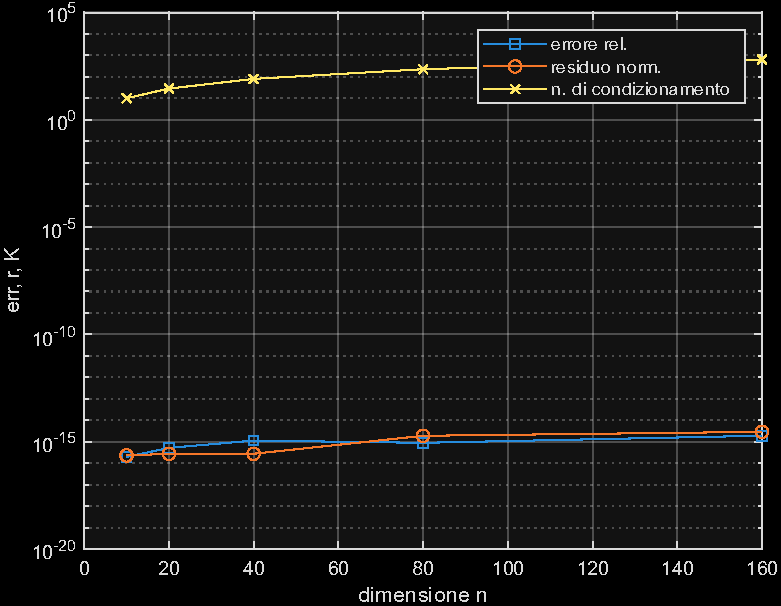
\includegraphics[width=.7\textwidth]{img/metodi-diretti.pdf}
        \caption{Andamento dell'errore relativo, del residuo normalizzato e del numero di condizionamento in funzione di $n$.}
    \end{figure}
\end{enumerate}